\chapter{Scelte progettuali}
\label{chap:scelte_progettuali}
Analizzando la scelta dei tool disponibili per il versioning, si evince che Git è il VCS più diffuso e più utilizzato\cite{gitmostused} dagli sviluppatori, è facile da utilizzare per i principianti ma allo stesso tempo supporta funzionalità avanzate per gli utenti più esperti. Per questo motivo si è deciso di ispirarsi al suo funzionamento per la realizzazione di \texttt{GGit}, mantenendo l'interfaccia utente esposta da Git, seppur in forma ridotta, per creare un'esperienza di utilizzo familiare.
\section{Strutture dati di GGit}
\label{sec:strutture_dati}
Git è nato come un semplice content-addressable filesystem, ovvero un sistema di storage basato su una relazione chiave-valore, nel quale è possibile archiviare qualsiasi tipo di contenuto digitale. Essenzialmente, l'azione di base che Git esegue è quella di memorizzare i contenuti di un file associandoli ad un hash calcolato su di essi: questa è la chiave che può essere utilizzata per accedere ai dati salvati.

L'hash di ogni oggetto (nomenclatura utilizzata per file e altre entità descritte in seguito), è calcolato usando l'algoritmo SHA-1, una funzione di hashing che genera un hash di 20 byte.
Pur essendo un algoritmo di hashing crittografico, SHA-1 non è sicuro, in quanto è stato provato che è possibile generare collisioni\cite{sha1collision} (ovvero due input che generano lo stesso hash).
Tuttavia, per l'utilizzo al quale è destinato all'interno di un VCS (cioè identificare univocamente il contenuto di un file) la complessità di SHA-1 è sufficiente, in quanto, nel peggior caso trovato, è stato necessario effettuare $2^{61}$ operazioni per ottenere una collisione\cite{collisionprob}.

Git si basa su 5 tipi di oggetti:
\begin{itemize}
    \item blob: oggetti che rappresentano un file;
    \item tree: oggetti che rappresentano una directory;
    \item commit: oggetti che pongono un particolare tree (la root directory) nella storia della repository, associando un commit padre, un timestamp e un messaggio che descrive le modifiche apportate;
    \item tag: un container che riferisce un altro oggetto, usato prevalentemente per dare un nome a un commit;
    \item packfile: una versione compressa di una serie di oggetti.
\end{itemize}
Il contenuto che verrà dato come input alla funzione di hash sarà una stringa che racchiude le caratteristiche dello specifico oggetto, fattore che aiuta a ridurre ulteriormente la probabilità di collisioni.

Si è deciso di strutturare il modello del dominio di GGit considerando i primi tre tipi di oggetti: blob, tree e commit.
Di seguito viene illustrato come vengono calcolati gli hash di ogni tipo di oggetto.

\subsection{Blob}
Un file è rappresentato da un blob, per calcolarne l'hash si considera la caratteristica principale, ovvero il suo contenuto, che viene considerato in byte sia per file in puro testo ASCII che binari.
Viene poi calcolata la lunghezza in byte del contenuto e il valore risultante viene concatenato con la stringa \texttt{"blob "}, seguita da un carattere NULL il tutto seguito dal contenuto del file:
\begin{minted}[bgcolor=lightgray,framesep=2mm,baselinestretch=1.2,fontsize=\footnotesize]{bash}
blob <file_length>\0<file_content>
\end{minted}
\subsection{Tree}
Un tree è essenzialmente una collezione di blob e tree, la funzione di un tree è associare a blob e tree un nome e una stringa che esprime i permessi sul file.


I permessi sono espressi in modo analogo alla modalità utilizzata dai sistemi UNIX, ovvero tre caratteri ottali che indicano i permessi di lettura, scrittura e esecuzione per il proprietario, il gruppo e gli altri utenti, una cifra ottale che rappresenterebbe i bit setuid, setgid e sticky (ignorati da Git) e altri tre caratteri ottali che indicano la POSIX mode\cite{gitmodes} dell'oggetto:
\begin{itemize}
    \item 04 per directory;
    \item 10 per file regolari;
    \item 12 per link simbolico;
    \item 16 per Git link o sottomoduli, non presente tra le classiche POSIX modes (non supportati da GGit).
\end{itemize}
L'hash di un tree viene calcolato in modo analogo a quello di un blob:
\begin{minted}[bgcolor=lightgray,framesep=2mm,baselinestretch=1.2,fontsize=\footnotesize]{bash}
tree <tree_length>\0<tree_content>
\end{minted}
dove \texttt{tree\_length} è la lunghezza in byte del \texttt{tree\_content}, che è una lista di oggetti, in ordine alfabetico per nome, nel seguente formato:
\begin{minted}[bgcolor=lightgray,framesep=2mm,baselinestretch=1.2,fontsize=\footnotesize]{bash}
<object_mode> <object_name>\0<object_hash>
\end{minted}
La stringa \texttt{object\_name} è il nome del file o directory e \text{object\_hash} l'hash dell'oggetto corrispondente.
La \texttt{object\_mode} è la stringa di sei caratteri ottali che identifica il tipo e i permessi dell'oggetto descritta in precedenza, questa stringa in GGit può assumere i seguenti valori:
\begin{itemize}
    \item 100644 per file regolari;
    \item 100755 per file eseguibili;
    \item 040000 per directory (altri tree);
    \item 120000 per link simbolici,
\end{itemize}
nel caso in cui la stringa abbia zeri iniziali, questi vengono troncati (regola applicabile soltanto nel caso delle directory).
\subsection{Commit}
La funzione principale di un commit è quella di associare lo stato corrente dell'area di commit a un punto nella storia della repository e facilitare la reperibilità di un particolare stato della repository.
L'area di commit, in GGit chiamata \texttt{stash}, è essenzialmente una lista di file che verranno aggiunti al prossimo commit.
Per calcolare l'hash di un commit si procede in modo analogo a quello degli altri tipi di oggetti:
\begin{minted}[bgcolor=lightgray,framesep=2mm,baselinestretch=1.2,fontsize=\footnotesize]{bash}
commit <commit_length>\0<commit_content>
\end{minted}
dove \texttt{commit\_length} è la lunghezza in byte del \texttt{commit\_content}, che è una stringa formattata come segue:
\begin{minted}[bgcolor=lightgray,framesep=2mm,baselinestretch=1.2,fontsize=\footnotesize]{text}
tree <tree_hash>
parent <parent_hash>
author <author_name> <<author_email>> <author_timestamp> <timezone>
committer <committer_name> <<committer_email>> <committer_timestamp> <timezone>

<commit_message>
\end{minted}
Il \texttt{tree\_hash} è l'hash del tree che rappresenta la root directory dell'area di lavoro, il \texttt{parent\_hash} è l'hash del commit padre, ovvero il commit dal quale è stato creato il commit corrente, se il commit è il primo della storia della repository, questo campo è omesso.
Le due linee successive contengono le informazioni che identificano rispettivamente l'utente che ha implementato le modifiche (author) e l'utente che ha creato il commit (committer). A oggi GGit non supporta la possibilità di applicare patch a commit passati come Git\cite{gitdocsauthcomm}, è però possibile, al momento della creazione del commit, specificare un autore diverso dal committer, per dare credito all'effettivo autore del codice e non solo all'utente che lo ha accettato all'interno della repository.
Infine l'ultima riga è il messaggio associato al commit, stringa che idealmente descrive le modifiche che vengono implementate con il commit.
\section{Database}
\label{sec:database}
I tipi di oggetti in gioco hanno un alto livello di interconnessione tra di loro: ogni commit è relativo a un tree, un tree può contenere molteplici blob e tree e un tree diverso può contenere un sottoinsieme di blob e tree di un altro tree. Data questa caratteristica, si è scelto di utilizzare un database a grafi.

La gamma di diversi tipi di database a grafi è ampia (anche se non come nel caso dei database relazionali); si è scelto di utilizzare per questo progetto Neo4j, un database a grafi scalabile orizzontalmente del quale esiste una community edition totalmente opensource\cite{neo4jgit}. Neo4j è inoltre il database a grafi più utilizzato\cite{db-engines_2022}, con una vasta community di sviluppatori, il che aiuta in fase di sviluppo per trovare soluzioni ad eventuali problemi.

Un'altra caratteristica che ha portato alla scelta di questo particolare database sono i tool a supporto dello sviluppo, come ad esempio Neo4j Desktop o Browser, che espongono una interfaccia grafica intuitiva per eseguire query e visualizzare rappresentazioni grafiche dei grafi risultanti; è disponibile inoltre Neo4j AuraDB che permette di effettuare il deployment di un database a grafi in cloud, permettendo quindi di creare repository condivise senza necessità di gestire infrastrutture server.

\subsection{Sviluppo del modello di dati}
\label{sec:datamodel}
Il modello di dati è stato sviluppato per poter rappresentare in modo completo tutti i tipi di oggetti presenti in GGit e grazie alla caratteristica schema-less dei database a grafi, sarà possibile aggiungere nuovi tipi di oggetti o caratteristiche al modello del dominio senza intaccare maggiormente la struttura preesistente.

Anche se il database scelto è schema-less, è comunque buona pratica definire e documentare in modo preciso il modello dei dati, così da evitare in futuro di fare scelte incompatibili con il modello preesistente.

Per sviluppare il modello dei dati è possibile sfruttare l'approccio "whiteboard", che permette di rappresentare il modello in modo grafico per esprimere ad alto livello le entità e le relazioni in gioco per poi formalizzare la struttura senza dover convertire le decisioni prese in tabelle.
\begin{figure}[H]
    \centering
    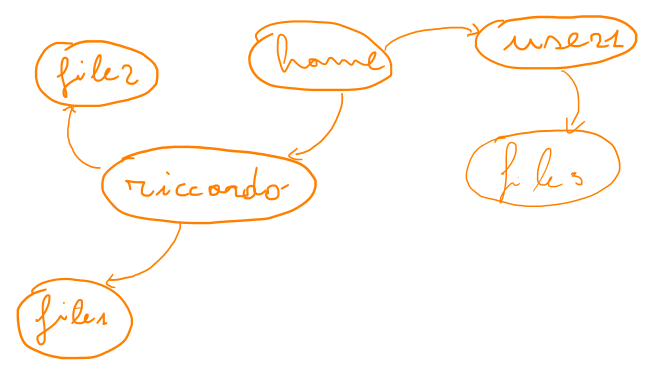
\includegraphics[width=15cm]{./immagini/whiteboard_sketch.png}
    \caption{Whiteboard sketch della struttura di un'ipotetica repository}
\end{figure}
Dopo aver creato il cosiddetto "whiteboard model" si procede alla formalizzazione delle entità e relazioni individuate, etichettando con label le entità e relazioni e associandovi tutte le proprietà.
\begin{figure}[H]
    \centering
    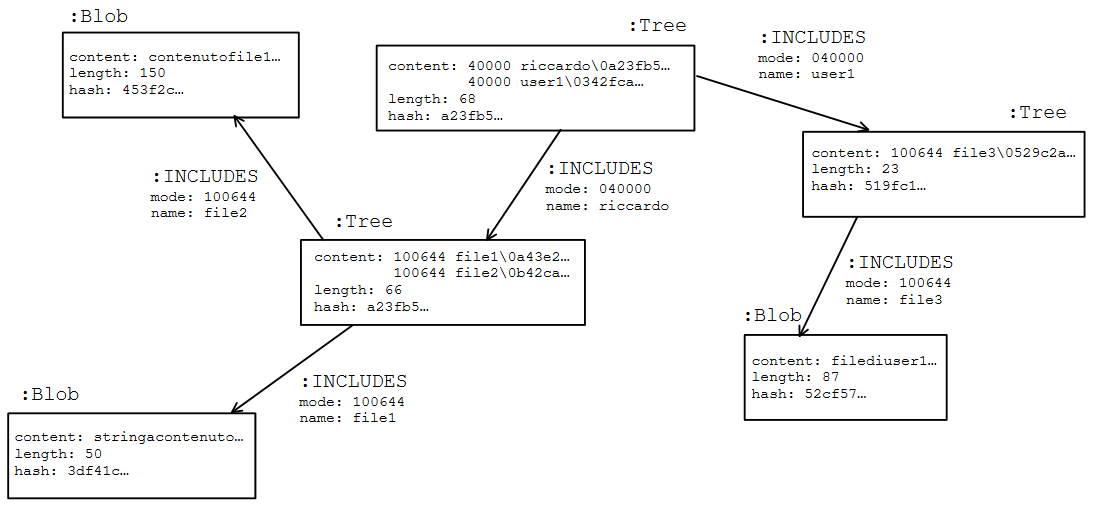
\includegraphics[width=15cm]{./immagini/whiteboard_formal.png}
    \caption{Formalizzazione dello sketch con proprietà e label}
\end{figure}
Come si nota dalla figura precedente si è deciso di assegnare i label (case sensitive) \texttt{:Tree} e \texttt{:Blob} alle rispettive entità, si individuano inoltre le seguenti proprietà per entrambi i tipi di oggetti:
\begin{itemize}
    \item \texttt{hash}: identificatore univoco dell'oggetto, calcolato con l'algoritmo SHA-1;
    \item \texttt{size}: dimensione in byte del contenuto;
    \item \texttt{content}: contenuto dell'oggetto, come descritti sopra.
\end{itemize}

Per quanto riguarda le relazioni, in questo sottoinsieme del modello se ne individua soltanto una: il label \texttt{:INCLUDES} indica che un oggetto ne contiene un altro. Le relazioni sono ordinate e nel caso di \texttt{:INCLUDES} il nodo di partenza è sempre un \texttt{:Tree} e il nodo di arrivo può essere sia un \texttt{:Tree} che un \texttt{:Blob}.
Si denotano inoltre due proprietà per questa relazione:
\begin{itemize}
    \item \texttt{name}: nome del file o della directory;
    \item \texttt{mode}: GGit mode dell'oggetto, può assumere il valore "040000" se il nodo di arrivo ha il label \texttt{:Tree} e i valori {"100644", "100755", "120000"} se il nodo di arrivo ha il label \texttt{:Blob}.
\end{itemize}

È stata fatta la scelta di associare le proprietà \texttt{name} e \texttt{mode} alla relazione e non al nodo in quanto rispecchia correttamente il modello dei dati definito: un oggetto \texttt{blob}, così come un \texttt{tree}, non ha un nome o una mode associati fino al momento in cui viene inserito all'interno di un \texttt{tree}.

Sotto viene mostrato il whiteboard sketch relativo al modello dei \texttt{commit} e degli \texttt{user}, e come possono essere collegati tra di loro:
\begin{figure}[H]
    \centering
    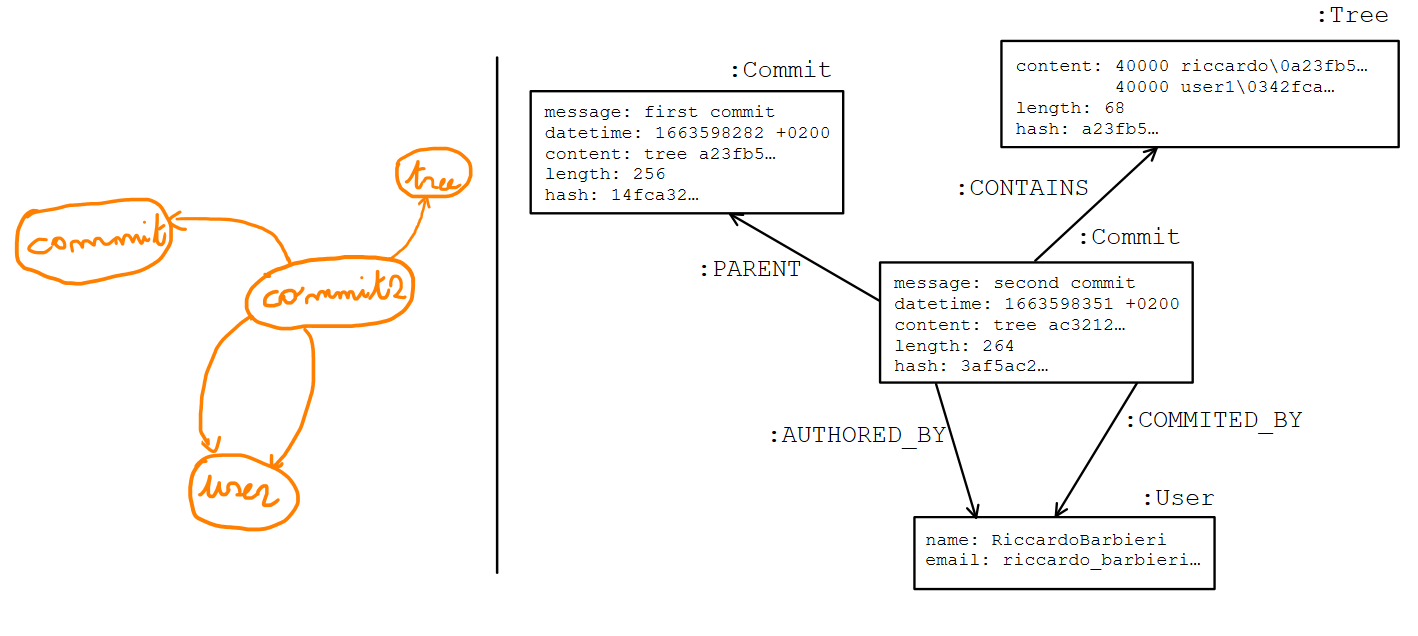
\includegraphics[width=15cm]{./immagini/whiteboard_commit.png}
    \caption{Whiteboard sketch del modello dei commit e degli user}
\end{figure}
In questa sezione del modello si individuano due nuove entità, \texttt{:Commit}, che è identificata dalle seguenti proprietà:
\begin{itemize}
    \item \texttt{message}: messaggio del commit;
    \item \texttt{datetime}: momento di creazione del commit (UNIX timestamp) e fuso orario (in ore dal UTC);
    \item \texttt{content}: stringa che rappresenta il commit (quella che viene data come input all'algoritmo di hashing).
    \item \texttt{length}: lunghezza del content.
    \item \texttt{hash}: identificatore univoco del commit, calcolato come descritto sopra,
\end{itemize}
e \texttt{:User}, identificata dalle seguenti proprietà:
\begin{itemize}
    \item \texttt{name}: nome dell'utente;
    \item \texttt{email}: email dell'utente;
\end{itemize}
Si identificano inoltre nuove relazioni: \texttt{:COMMITTED\_BY} e \texttt{:AUTHORED\_BY} che indicano rispettivamente il committer e l'autore di un commit; \texttt{:PARENT} che parte da un commit e punta al commit padre e infine \texttt{:CONTAINS} che parte da un commit e punta ad un oggetto \texttt{tree} che rappresenta lo stato della repository al momento del commit.

Come dimostrato, il modello whiteboard è estremamente utile per formalizzare le entità e relazioni in gioco e per individuare le proprietà da associare ad esse, data la natura ad alto livello di questo approccio è molto semplice passare da un idea, o uno sketch, a una definizione formale del modello dei dati.
\section{Stato della repository}
\label{sec:stato}
In questa sezione verranno descritte le modalità di gestione dello stato della repository, che comprende la lista dei file cosiddetti "tracked"; la lista dei file "stashed" e la gestione delle differenze dei file dell'ultima versione.

\subsection{Stash e tracking}
\label{subsec:stash}
Una delle funzioni fondamentali che GGit utilizza per tenere traccia della storia di una repository è l'area di \texttt{stash}, questa è l'area che raccoglie la lista dei file che verranno aggiunti al prossimo commit.
Questa area è strettamente legata alla lista dei file tracked, che sono quei file che un qualsiasi punto nella storia della repository sono stati aggiunti all'area di stash.

Si è scelto di mantenere l'area di stash e tracking nella repository stessa, in memoria locale, in modo da evitare di dover sostenere una connessione al database per operazioni che possono essere ripetute frequentemente.

\subsection{Differenze tra versioni di file}
\label{subsec:differenze}
GGit è in grado di riportare quali file sono stati modificati rispetto all'ultima versione, nella versione corrente dell'applicazione questa funzione è utile soltanto ai fini di un particolare comando (descritto successivamente) ma si è deciso di aggiungere questa funzionalità a supporto di future operazioni, come ad esempio la gestione di conflitti durante il merge automatico di versione differenti di uno stesso file.

\section{Gestione del server Neo4j}
Inizialmente si era pensato di includere una distribuzione del server Neo4j all'interno del package dell'applicazione, in modo da non dover richiedere all'utente di installare il server autonomamente, tuttavia si è scelto di istruire l'utente a installare una versione del server Neo4j, la directory dell'installazione andrà poi specificata all'interno di una variabile d'ambiente chiamata \texttt{"NEO4J\_HOME"}, variabile che verrà utilizzata per reperire l'installazione e copiarla all'interno di ciascuna repository; il database copiato viene poi inizializzato.

È stata fatta questa scelta per permettere di utilizzare la versione community del server di Neo4j per repository locali, versione che non permette di creare multipli database associati allo stesso server, è comunque possibile utilizzare una versione enterprise del server, ma richiede configurazione aggiuntiva (discussa nelle \hyperref[sec:impostazioni]{Impostazioni di configurazione}).
Inoltre è possibile connettersi ad un server Neo4j remoto, in questo caso è necessario specificare l'indirizzo del server e le credenziali di accesso attraverso le impostazioni di configurazione.

\section{Interfaccia utente}
\label{sec:interfaccia}
L'interfaccia utente di \texttt{GGit} è ispirata a quella di \texttt{Git}, del quale si è deciso di implementare un sottoinsieme ridotto di comandi, ovvero quelli essenziali al funzionamento di base di un VCS:
\begin{itemize}
    \item \texttt{init};
    \item \texttt{add};
    \item \texttt{mv};
    \item \texttt{rm};
    \item \texttt{commit};
    \item \texttt{status};
    \item \texttt{config};
    \item \texttt{log}.
\end{itemize}

\subsection{Gestione della repository}
Questi sono i comandi per gestire la repository.

\subsubsection{Init}
Il comando \texttt{ggit init} crea una nuova repository, in particolare viene create la directory \texttt{.ggit} all'interno della directory nella quale viene chiamato il comando, si è però deciso di permettere all'utente di specificare la directory da inizializzare con il comando \texttt{ggit init <path>}, in questo modo è possibile creare una repository all'interno di una directory diversa dalla corrente.

Dopo aver creato la directory, vengono inizializzati i file di configurazione e dello stato e vengono impostate alcune configurazioni di base, viene inoltre richiesto interattivamente all'utente di inserire username e email, che verranno utilizzati per i commit.
Viene poi inizializzato lo stato della repository, reperita l'installazione di Neo4j e impostate le impostazioni relative a username, password e nome, versione e posizione del database.

\subsubsection{Config}
Il comando \texttt{ggit config} permette di gestire le impostazioni di configurazione, in particolare è possibile visualizzare le impostazioni correnti, impostare nuove impostazioni e rimuovere impostazioni esistenti.

Questo comando offre i seguenti parametri:
\begin{itemize}
    \item \texttt{-{}-list} per visualizzare tutte le impostazioni correnti;
    \item \texttt{-{}-get <key>} per visualizzare il valore di una impostazione;
    \item \texttt{-{}-set <key> <value>} per impostare il valora di una impostazione, se non esiste viene aggiunta;
    \item \texttt{-{}-unset <key>} per rimuovere una impostazione.
\end{itemize}

\subsection{Gestione dei file}
I seguenti comandi sono disponibili all'utente per modificare lo stato della repository, aggiungendo rimuovendo e spostando file.

Tutti i comandi in questa categoria supportano l'utilizzo da qualsiasi sottodirectory della repository, tenendo conto della relatività degli eventuali path specificati.
\subsubsection{Add}
Il comando \texttt{ggit add} permette di aggiungere un lista di file e/o directory all'area di \texttt{stash} della repository; ogni volta che un file viene aggiunto, viene anche inserito nella lista dei file tracked, nel caso delle directory vengono aggiunti tutti i file contenuti nella directory stessa e in tutte le sottodirectory.

Il comando offre un solo parametro, obbligatorio, che accetta valori multipli sotto forma di lista separata da spazi, questi sono le stringhe che verranno interpretate come path.

\subsubsection{Mv}
Il comando \texttt{ggit mv} permette di spostare un file o una directory da una posizione all'altra, in questo caso il file viene effettivamente spostato nel file system e viene aggiornato il path del file nella lista dei file tracked e dello stash.

Il comando accetta due parametri, obbligatori, che accettano rispettivamente un solo valore che verrà interpretato come path, il primo è il file o la directory di partenza e il secondo la destinazione.

\subsubsection{Rm}
Il comando \texttt{ggit rm} permette di rimuovere un file o una directory, specificati come parametri, dalla lista dei file tracked e dello stash, in questo caso il file viene rimosso dal file system.

Così come il comando \texttt{add}, anche questo comando supporta l'utilizzo di valori multipli, separati da spazi, per specificare più file o directory da rimuovere.

\subsection{Gestione della storia}
\subsubsection{Commit}
Il comando \texttt{ggit commit} permette di creare un nuovo commit partendo dallo stato corrente dello stash della repository.

Inizialmente viene creato un nuovo oggetto tree, partendo dallo stash della repository. Dopodiché vengono interpretate le opzioni passate al comando, in particolare è possibile specificare:
\begin{itemize}
    \item \texttt{-m} o \texttt{-{}-message}: specifica il messaggio del commit;
    \item \texttt{-f} o \texttt{-{}-file}: specifica il nome del file dal quale leggere il messaggio di commit, mutualmente esclusivo con \texttt{-m};
    \item \texttt{-{}-author}: specifica l'autore del commit, nel formato \texttt{nome,email} per effettuare l'override dell'autore di default;
    \item \texttt{-{}-date}: specifica la data, nel formato \texttt{YYYY-MM-DDTHH:mm:SS+HH:mm} per effettuare l'override della data corrente.
\end{itemize}
Dopo aver valutato e interpretato le opzioni, viene recuperato dalle impostazioni di configurazione l'hash dell'ultimo commit, con il quale si ottiene dal database l'oggetto commit associato che viene assegnato al nuovo commit, se questa impostazione è vuota o non presente, significa che il commit che viene effettuato è il primo e non necessita un parent.

Infine viene effettivamente aggiunto il commit al database, aggiornata l'impostazione relativa all'ultimo commit e viene svuotato lo stash.

\subsection{Visualizzazione dello stato}
\subsubsection{Status}
Il comando \texttt{ggit status} permette di visualizzare un riassunto dello stato corrente della directory, in particolare vengono mostrate tre liste di file.
La prima lista elenca i file che sono al momento nell'area di \texttt{stash} e quindi verranno aggiunti al prossimo commit.
La seconda lista mostra i file che sono stati modificati rispetto al commit precedente, sono stati aggiunti, a un certo punto nella storia della repository, all'area di \texttt{tracking} e non sono ancora nell'area di \texttt{stash}. Infine la terza lista contiene i file che sono stati creati ma non sono mai stati aggiunti all'area di \texttt{stash} e quindi non sono ancora nel tracking della repository.

\subsubsection{Log}
Il comando \texttt{ggit log} permette di visualizzare lo storico dei commit della repository, stampa una lista dei commit più recenti, mostrando il loro hash, l'autore, la data di creazione e il messaggio di commit.

Il comando supporta una opzione \texttt{-d} o \texttt{-{}-depth} che permette di specificare il numero di commit da visualizzare, il valore di default è impostato a 5.

\section{Impostazioni di configurazione}
\label{sec:impostazioni}
Le impostazioni di configurazione sono una serie di entry chiave-valore, vengono utilizzate dall'applicazione per salvare e ottenere informazioni relative alla configurazione della repository e del database.

Tutte queste impostazioni possono essere aggiunte o modificate manualmente attraverso il comando \texttt{ggit config}.

\subsection{Configurazione della repository}
Alla versione corrente, le impostazioni di configurazione della repository sono le seguenti:
\begin{itemize}
    \item \texttt{"repository.path"}: path che punta alla root directory della repository;
    \item \texttt{"HEAD"}: contiene l'hash dell'ultimo commit effettuato, se non è presente o è impostato a \texttt{"None"} significa che non è ancora stato effettuato nessun commit;
    \item \texttt{"user.name"} e \texttt{"user.email"}: nome dell'utente e email utilizzati per i commit.
\end{itemize}

\subsection{Configurazione del database}
\begin{itemize}
    \item \texttt{"database.username"} e \texttt{"database.password"}, che contengono le credenziali di accesso al database di default;
    \item \texttt{"database.name"}, contiene il nome di default del database nella community edition;
    \item \texttt{"database.path"}, salva il path alla directory di installazione di Neo4j, ottenuto tramite la variabile d'ambiente \texttt{"NEO4J\_HOME"}.
\end{itemize}

Le impostazioni del database vengono inizializzate automaticamente ai valori utili per la community edition, per utilizzarne una enterprise è necessario modificare manualmente le variabile\texttt{"database.username"} e \texttt{"database.password"} con le credenziali personalizzate del database, mentre la variabile \texttt{"database.name"} deve essere impostata al nome del database che si vuole utilizzare.